\documentclass[1p]{elsarticle_modified}
%\bibliographystyle{elsarticle-num}

%\usepackage[colorlinks]{hyperref}
%\usepackage{abbrmath_seonhwa} %\Abb, \Ascr, \Acal ,\Abf, \Afrak
\usepackage{amsfonts}
\usepackage{amssymb}
\usepackage{amsmath}
\usepackage{amsthm}
\usepackage{scalefnt}
\usepackage{amsbsy}
\usepackage{kotex}
\usepackage{caption}
\usepackage{subfig}
\usepackage{color}
\usepackage{graphicx}
\usepackage{xcolor} %% white, black, red, green, blue, cyan, magenta, yellow
\usepackage{float}
\usepackage{setspace}
\usepackage{hyperref}

\usepackage{tikz}
\usetikzlibrary{arrows}

\usepackage{multirow}
\usepackage{array} % fixed length table
\usepackage{hhline}

%%%%%%%%%%%%%%%%%%%%%
\makeatletter
\renewcommand*\env@matrix[1][\arraystretch]{%
	\edef\arraystretch{#1}%
	\hskip -\arraycolsep
	\let\@ifnextchar\new@ifnextchar
	\array{*\c@MaxMatrixCols c}}
\makeatother %https://tex.stackexchange.com/questions/14071/how-can-i-increase-the-line-spacing-in-a-matrix
%%%%%%%%%%%%%%%

\usepackage[normalem]{ulem}

\newcommand{\msout}[1]{\ifmmode\text{\sout{\ensuremath{#1}}}\else\sout{#1}\fi}
%SOURCE: \msout is \stkout macro in https://tex.stackexchange.com/questions/20609/strikeout-in-math-mode

\newcommand{\cancel}[1]{
	\ifmmode
	{\color{red}\msout{#1}}
	\else
	{\color{red}\sout{#1}}
	\fi
}

\newcommand{\add}[1]{
	{\color{blue}\uwave{#1}}
}

\newcommand{\replace}[2]{
	\ifmmode
	{\color{red}\msout{#1}}{\color{blue}\uwave{#2}}
	\else
	{\color{red}\sout{#1}}{\color{blue}\uwave{#2}}
	\fi
}

\newcommand{\Sol}{\mathcal{S}} %segment
\newcommand{\D}{D} %diagram
\newcommand{\A}{\mathcal{A}} %arc


%%%%%%%%%%%%%%%%%%%%%%%%%%%%%5 test

\def\sl{\operatorname{\textup{SL}}(2,\Cbb)}
\def\psl{\operatorname{\textup{PSL}}(2,\Cbb)}
\def\quan{\mkern 1mu \triangleright \mkern 1mu}

\theoremstyle{definition}
\newtheorem{thm}{Theorem}[section]
\newtheorem{prop}[thm]{Proposition}
\newtheorem{lem}[thm]{Lemma}
\newtheorem{ques}[thm]{Question}
\newtheorem{cor}[thm]{Corollary}
\newtheorem{defn}[thm]{Definition}
\newtheorem{exam}[thm]{Example}
\newtheorem{rmk}[thm]{Remark}
\newtheorem{alg}[thm]{Algorithm}

\newcommand{\I}{\sqrt{-1}}
\begin{document}

%\begin{frontmatter}
%
%\title{Boundary parabolic representations of knots up to 8 crossings}
%
%%% Group authors per affiliation:
%\author{Yunhi Cho} 
%\address{Department of Mathematics, University of Seoul, Seoul, Korea}
%\ead{yhcho@uos.ac.kr}
%
%
%\author{Seonhwa Kim} %\fnref{s_kim}}
%\address{Center for Geometry and Physics, Institute for Basic Science, Pohang, 37673, Korea}
%\ead{ryeona17@ibs.re.kr}
%
%\author{Hyuk Kim}
%\address{Department of Mathematical Sciences, Seoul National University, Seoul 08826, Korea}
%\ead{hyukkim@snu.ac.kr}
%
%\author{Seokbeom Yoon}
%\address{Department of Mathematical Sciences, Seoul National University, Seoul, 08826,  Korea}
%\ead{sbyoon15@snu.ac.kr}
%
%\begin{abstract}
%We find all boundary parabolic representation of knots up to 8 crossings.
%
%\end{abstract}
%\begin{keyword}
%    \MSC[2010] 57M25 
%\end{keyword}
%
%\end{frontmatter}

%\linenumbers
%\tableofcontents
%
\newcommand\colored[1]{\textcolor{white}{\rule[-0.35ex]{0.8em}{1.4ex}}\kern-0.8em\color{red} #1}%
%\newcommand\colored[1]{\textcolor{white}{ #1}\kern-2.17ex	\textcolor{white}{ #1}\kern-1.81ex	\textcolor{white}{ #1}\kern-2.15ex\color{red}#1	}

{\Large $\underline{12a_{0324}~(K12a_{0324})}$}

\setlength{\tabcolsep}{10pt}
\renewcommand{\arraystretch}{1.6}
\vspace{1cm}\begin{tabular}{m{100pt}>{\centering\arraybackslash}m{274pt}}
\multirow{5}{120pt}{
	\centering
	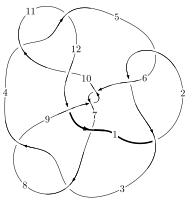
\includegraphics[width=112pt]{../../../GIT/diagram.site/Diagrams/png/1125_12a_0324.png}\\
\ \ \ A knot diagram\footnotemark}&
\allowdisplaybreaks
\textbf{Linearized knot diagam} \\
\cline{2-2}
 &
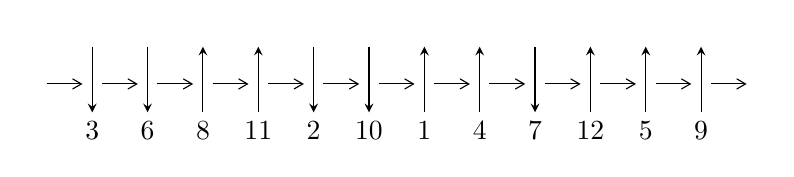
\begin{tikzpicture}[x=20pt, y=17pt]
	% nodes
	\node (C0) at (0, 0) {};
	\node (C1) at (1, 0) {};
	\node (C1U) at (1, +1) {};
	\node (C1D) at (1, -1) {3};

	\node (C2) at (2, 0) {};
	\node (C2U) at (2, +1) {};
	\node (C2D) at (2, -1) {6};

	\node (C3) at (3, 0) {};
	\node (C3U) at (3, +1) {};
	\node (C3D) at (3, -1) {8};

	\node (C4) at (4, 0) {};
	\node (C4U) at (4, +1) {};
	\node (C4D) at (4, -1) {11};

	\node (C5) at (5, 0) {};
	\node (C5U) at (5, +1) {};
	\node (C5D) at (5, -1) {2};

	\node (C6) at (6, 0) {};
	\node (C6U) at (6, +1) {};
	\node (C6D) at (6, -1) {10};

	\node (C7) at (7, 0) {};
	\node (C7U) at (7, +1) {};
	\node (C7D) at (7, -1) {1};

	\node (C8) at (8, 0) {};
	\node (C8U) at (8, +1) {};
	\node (C8D) at (8, -1) {4};

	\node (C9) at (9, 0) {};
	\node (C9U) at (9, +1) {};
	\node (C9D) at (9, -1) {7};

	\node (C10) at (10, 0) {};
	\node (C10U) at (10, +1) {};
	\node (C10D) at (10, -1) {12};

	\node (C11) at (11, 0) {};
	\node (C11U) at (11, +1) {};
	\node (C11D) at (11, -1) {5};

	\node (C12) at (12, 0) {};
	\node (C12U) at (12, +1) {};
	\node (C12D) at (12, -1) {9};
	\node (C13) at (13, 0) {};

	% arrows
	\draw[->,>={angle 60}]
	(C0) edge (C1) (C1) edge (C2) (C2) edge (C3) (C3) edge (C4) (C4) edge (C5) (C5) edge (C6) (C6) edge (C7) (C7) edge (C8) (C8) edge (C9) (C9) edge (C10) (C10) edge (C11) (C11) edge (C12) (C12) edge (C13) ;	\draw[->,>=stealth]
	(C1U) edge (C1D) (C2U) edge (C2D) (C3D) edge (C3U) (C4D) edge (C4U) (C5U) edge (C5D) (C6U) edge (C6D) (C7D) edge (C7U) (C8D) edge (C8U) (C9U) edge (C9D) (C10D) edge (C10U) (C11D) edge (C11U) (C12D) edge (C12U) ;
	\end{tikzpicture} \\
\hhline{~~} \\& 
\textbf{Solving Sequence} \\ \cline{2-2} 
 &
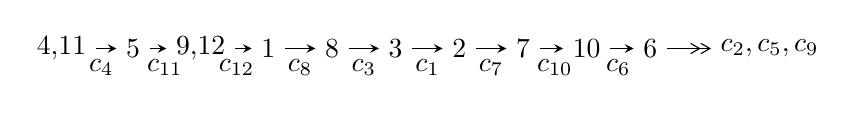
\begin{tikzpicture}[x=23pt, y=7pt]
	% node
	\node (A0) at (-1/8, 0) {4,11};
	\node (A1) at (1, 0) {5};
	\node (A2) at (33/16, 0) {9,12};
	\node (A3) at (25/8, 0) {1};
	\node (A4) at (33/8, 0) {8};
	\node (A5) at (41/8, 0) {3};
	\node (A6) at (49/8, 0) {2};
	\node (A7) at (57/8, 0) {7};
	\node (A8) at (65/8, 0) {10};
	\node (A9) at (73/8, 0) {6};
	\node (C1) at (1/2, -1) {$c_{4}$};
	\node (C2) at (3/2, -1) {$c_{11}$};
	\node (C3) at (21/8, -1) {$c_{12}$};
	\node (C4) at (29/8, -1) {$c_{8}$};
	\node (C5) at (37/8, -1) {$c_{3}$};
	\node (C6) at (45/8, -1) {$c_{1}$};
	\node (C7) at (53/8, -1) {$c_{7}$};
	\node (C8) at (61/8, -1) {$c_{10}$};
	\node (C9) at (69/8, -1) {$c_{6}$};
	\node (A10) at (11, 0) {$c_{2},c_{5},c_{9}$};

	% edge
	\draw[->,>=stealth]	
	(A0) edge (A1) (A1) edge (A2) (A2) edge (A3) (A3) edge (A4) (A4) edge (A5) (A5) edge (A6) (A6) edge (A7) (A7) edge (A8) (A8) edge (A9) ;
	\draw[->>,>={angle 60}]	
	(A9) edge (A10);
\end{tikzpicture} \\ 

\end{tabular} \\

\footnotetext{
The image of knot diagram is generated by the software ``\textbf{Draw programme}" developed by Andrew Bartholomew(\url{http://www.layer8.co.uk/maths/draw/index.htm\#Running-draw}), where we modified some parts for our purpose(\url{https://github.com/CATsTAILs/LinksPainter}).
}\phantom \\ \newline 
\centering \textbf{Ideals for irreducible components\footnotemark of $X_{\text{par}}$} 
 
\begin{align*}
I^u_{1}&=\langle 
-5.97705\times10^{454} u^{150}+5.44321\times10^{453} u^{149}+\cdots+1.74550\times10^{455} b+3.85569\times10^{456},\\
\phantom{I^u_{1}}&\phantom{= \langle  }1.24527\times10^{457} u^{150}-4.69754\times10^{456} u^{149}+\cdots+1.02984\times10^{457} a-1.13363\times10^{459},\\
\phantom{I^u_{1}}&\phantom{= \langle  }u^{151}- u^{150}+\cdots-347 u+59\rangle \\
I^u_{2}&=\langle 
-6960094 u^{37}-14517025 u^{36}+\cdots+2084882 b+33128019,\\
\phantom{I^u_{2}}&\phantom{= \langle  }100284480 u^{37}+64266775 u^{36}+\cdots+2084882 a-144370152,\;u^{38}-10 u^{36}+\cdots-2 u+1\rangle \\
\\
\end{align*}
\raggedright * 2 irreducible components of $\dim_{\mathbb{C}}=0$, with total 189 representations.\\
\footnotetext{All coefficients of polynomials are rational numbers. But the coefficients are sometimes approximated in decimal forms when there is not enough margin.}
\newpage
\renewcommand{\arraystretch}{1}
\centering \section*{I. $I^u_{1}= \langle -5.98\times10^{454} u^{150}+5.44\times10^{453} u^{149}+\cdots+1.75\times10^{455} b+3.86\times10^{456},\;1.25\times10^{457} u^{150}-4.70\times10^{456} u^{149}+\cdots+1.03\times10^{457} a-1.13\times10^{459},\;u^{151}- u^{150}+\cdots-347 u+59 \rangle$}
\flushleft \textbf{(i) Arc colorings}\\
\begin{tabular}{m{7pt} m{180pt} m{7pt} m{180pt} }
\flushright $a_{4}=$&$\begin{pmatrix}1\\0\end{pmatrix}$ \\
\flushright $a_{11}=$&$\begin{pmatrix}0\\u\end{pmatrix}$ \\
\flushright $a_{5}=$&$\begin{pmatrix}1\\- u^2\end{pmatrix}$ \\
\flushright $a_{9}=$&$\begin{pmatrix}-1.20919 u^{150}+0.456142 u^{149}+\cdots-509.338 u+110.078\\0.342427 u^{150}-0.0311843 u^{149}+\cdots+107.848 u-22.0893\end{pmatrix}$ \\
\flushright $a_{12}=$&$\begin{pmatrix}u\\- u^3+u\end{pmatrix}$ \\
\flushright $a_{1}=$&$\begin{pmatrix}0.0321236 u^{150}-0.160065 u^{149}+\cdots+124.646 u-27.6243\\0.560103 u^{150}-0.0814844 u^{149}+\cdots+176.427 u-36.0766\end{pmatrix}$ \\
\flushright $a_{8}=$&$\begin{pmatrix}-1.55162 u^{150}+0.487326 u^{149}+\cdots-617.186 u+132.167\\0.342427 u^{150}-0.0311843 u^{149}+\cdots+107.848 u-22.0893\end{pmatrix}$ \\
\flushright $a_{3}=$&$\begin{pmatrix}0.415768 u^{150}-0.161858 u^{149}+\cdots+122.308 u-31.5806\\-0.307673 u^{150}-0.0169399 u^{149}+\cdots-73.6657 u+14.9648\end{pmatrix}$ \\
\flushright $a_{2}=$&$\begin{pmatrix}-0.945289 u^{150}+0.0486104 u^{149}+\cdots-261.709 u+50.8717\\0.543340 u^{150}-0.113382 u^{149}+\cdots+173.488 u-36.6489\end{pmatrix}$ \\
\flushright $a_{7}=$&$\begin{pmatrix}0.234863 u^{150}+0.182289 u^{149}+\cdots+20.9259 u+2.63592\\-0.188680 u^{150}+0.118465 u^{149}+\cdots-71.2589 u+15.7347\end{pmatrix}$ \\
\flushright $a_{10}=$&$\begin{pmatrix}- u^3\\u^5- u^3+u\end{pmatrix}$ \\
\flushright $a_{6}=$&$\begin{pmatrix}0.597935 u^{150}+0.103993 u^{149}+\cdots+141.486 u-21.8592\\-0.407732 u^{150}+0.124190 u^{149}+\cdots-134.008 u+27.5308\end{pmatrix}$\\&\end{tabular}
\flushleft \textbf{(ii) Obstruction class $= -1$}\\~\\
\flushleft \textbf{(iii) Cusp Shapes $= 0.875815 u^{150}+0.572195 u^{149}+\cdots+22.1449 u+33.7195$}\\~\\
\newpage\renewcommand{\arraystretch}{1}
\flushleft \textbf{(iv) u-Polynomials at the component}\newline \\
\begin{tabular}{m{50pt}|m{274pt}}
Crossings & \hspace{64pt}u-Polynomials at each crossing \\
\hline $$\begin{aligned}c_{1}\end{aligned}$$&$\begin{aligned}
&u^{151}+59 u^{150}+\cdots-241657 u+120409
\end{aligned}$\\
\hline $$\begin{aligned}c_{2},c_{5}\end{aligned}$$&$\begin{aligned}
&u^{151}+3 u^{150}+\cdots+1193 u-347
\end{aligned}$\\
\hline $$\begin{aligned}c_{3},c_{8}\end{aligned}$$&$\begin{aligned}
&u^{151}+u^{150}+\cdots-3953 u-319
\end{aligned}$\\
\hline $$\begin{aligned}c_{4},c_{11}\end{aligned}$$&$\begin{aligned}
&u^{151}+u^{150}+\cdots-347 u-59
\end{aligned}$\\
\hline $$\begin{aligned}c_{6},c_{9}\end{aligned}$$&$\begin{aligned}
&u^{151}-6 u^{150}+\cdots+220218 u-26057
\end{aligned}$\\
\hline $$\begin{aligned}c_{7}\end{aligned}$$&$\begin{aligned}
&u^{151}-2 u^{150}+\cdots-15334096 u+82036477
\end{aligned}$\\
\hline $$\begin{aligned}c_{10}\end{aligned}$$&$\begin{aligned}
&u^{151}-73 u^{150}+\cdots+62943 u-3481
\end{aligned}$\\
\hline $$\begin{aligned}c_{12}\end{aligned}$$&$\begin{aligned}
&u^{151}+10 u^{150}+\cdots-194288 u-9629
\end{aligned}$\\
\hline
\end{tabular}\\~\\
\newpage\renewcommand{\arraystretch}{1}
\flushleft \textbf{(v) Riley Polynomials at the component}\newline \\
\begin{tabular}{m{50pt}|m{274pt}}
Crossings & \hspace{64pt}Riley Polynomials at each crossing \\
\hline $$\begin{aligned}c_{1}\end{aligned}$$&$\begin{aligned}
&y^{151}+85 y^{150}+\cdots+4342105053167 y-14498327281
\end{aligned}$\\
\hline $$\begin{aligned}c_{2},c_{5}\end{aligned}$$&$\begin{aligned}
&y^{151}-59 y^{150}+\cdots-241657 y-120409
\end{aligned}$\\
\hline $$\begin{aligned}c_{3},c_{8}\end{aligned}$$&$\begin{aligned}
&y^{151}-101 y^{150}+\cdots+16937937 y-101761
\end{aligned}$\\
\hline $$\begin{aligned}c_{4},c_{11}\end{aligned}$$&$\begin{aligned}
&y^{151}-73 y^{150}+\cdots+62943 y-3481
\end{aligned}$\\
\hline $$\begin{aligned}c_{6},c_{9}\end{aligned}$$&$\begin{aligned}
&y^{151}+94 y^{150}+\cdots-24366231410 y-678967249
\end{aligned}$\\
\hline $$\begin{aligned}c_{7}\end{aligned}$$&$\begin{aligned}
&y^{151}-58 y^{150}+\cdots+432393903636177302 y-6729983558571529
\end{aligned}$\\
\hline $$\begin{aligned}c_{10}\end{aligned}$$&$\begin{aligned}
&y^{151}+27 y^{150}+\cdots-2959833961 y-12117361
\end{aligned}$\\
\hline $$\begin{aligned}c_{12}\end{aligned}$$&$\begin{aligned}
&y^{151}-34 y^{150}+\cdots+5136926742 y-92717641
\end{aligned}$\\
\hline
\end{tabular}\\~\\
\newpage\flushleft \textbf{(vi) Complex Volumes and Cusp Shapes}
$$\begin{array}{c|c|c}  
\text{Solutions to }I^u_{1}& \I (\text{vol} + \sqrt{-1}CS) & \text{Cusp shape}\\
 \hline 
\begin{aligned}
u &= -0.266173 + 0.955595 I \\
a &= -0.039639 - 0.162305 I \\
b &= -1.001740 - 0.126781 I\end{aligned}
 & \phantom{-}0.0393853 + 0.0284279 I & \phantom{-0.000000 } 0 \\ \hline\begin{aligned}
u &= -0.266173 - 0.955595 I \\
a &= -0.039639 + 0.162305 I \\
b &= -1.001740 + 0.126781 I\end{aligned}
 & \phantom{-}0.0393853 - 0.0284279 I & \phantom{-0.000000 } 0 \\ \hline\begin{aligned}
u &= \phantom{-}0.180807 + 0.968414 I \\
a &= \phantom{-}0.186766 + 0.331168 I \\
b &= \phantom{-}0.627417 + 0.335459 I\end{aligned}
 & -1.59974 - 1.64062 I & \phantom{-0.000000 } 0 \\ \hline\begin{aligned}
u &= \phantom{-}0.180807 - 0.968414 I \\
a &= \phantom{-}0.186766 - 0.331168 I \\
b &= \phantom{-}0.627417 - 0.335459 I\end{aligned}
 & -1.59974 + 1.64062 I & \phantom{-0.000000 } 0 \\ \hline\begin{aligned}
u &= -0.301843 + 0.933657 I \\
a &= \phantom{-}0.663027 + 0.942111 I \\
b &= \phantom{-}1.332720 + 0.459969 I\end{aligned}
 & \phantom{-}6.43799 + 7.51813 I & \phantom{-0.000000 } 0 \\ \hline\begin{aligned}
u &= -0.301843 - 0.933657 I \\
a &= \phantom{-}0.663027 - 0.942111 I \\
b &= \phantom{-}1.332720 - 0.459969 I\end{aligned}
 & \phantom{-}6.43799 - 7.51813 I & \phantom{-0.000000 } 0 \\ \hline\begin{aligned}
u &= -0.767737 + 0.609881 I \\
a &= -0.64597 - 1.64540 I \\
b &= \phantom{-}0.729574 - 0.844251 I\end{aligned}
 & -4.00055 - 4.07728 I & \phantom{-0.000000 } 0 \\ \hline\begin{aligned}
u &= -0.767737 - 0.609881 I \\
a &= -0.64597 + 1.64540 I \\
b &= \phantom{-}0.729574 + 0.844251 I\end{aligned}
 & -4.00055 + 4.07728 I & \phantom{-0.000000 } 0 \\ \hline\begin{aligned}
u &= \phantom{-}0.910083 + 0.463641 I \\
a &= \phantom{-}0.028649 + 0.538279 I \\
b &= -0.115994 + 0.705686 I\end{aligned}
 & -0.568526 - 0.503686 I & \phantom{-0.000000 } 0 \\ \hline\begin{aligned}
u &= \phantom{-}0.910083 - 0.463641 I \\
a &= \phantom{-}0.028649 - 0.538279 I \\
b &= -0.115994 - 0.705686 I\end{aligned}
 & -0.568526 + 0.503686 I & \phantom{-0.000000 } 0\\
 \hline 
 \end{array}$$\newpage$$\begin{array}{c|c|c}  
\text{Solutions to }I^u_{1}& \I (\text{vol} + \sqrt{-1}CS) & \text{Cusp shape}\\
 \hline 
\begin{aligned}
u &= \phantom{-}0.966948 + 0.094963 I \\
a &= -1.59959 - 0.17797 I \\
b &= \phantom{-}1.361200 + 0.067293 I\end{aligned}
 & \phantom{-}6.58926 + 1.11575 I & \phantom{-0.000000 } 0 \\ \hline\begin{aligned}
u &= \phantom{-}0.966948 - 0.094963 I \\
a &= -1.59959 + 0.17797 I \\
b &= \phantom{-}1.361200 - 0.067293 I\end{aligned}
 & \phantom{-}6.58926 - 1.11575 I & \phantom{-0.000000 } 0 \\ \hline\begin{aligned}
u &= \phantom{-}0.592643 + 0.763145 I \\
a &= \phantom{-}0.845780 - 0.577160 I \\
b &= \phantom{-}0.871487 - 0.507063 I\end{aligned}
 & -3.36943 - 0.94507 I & \phantom{-0.000000 } 0 \\ \hline\begin{aligned}
u &= \phantom{-}0.592643 - 0.763145 I \\
a &= \phantom{-}0.845780 + 0.577160 I \\
b &= \phantom{-}0.871487 + 0.507063 I\end{aligned}
 & -3.36943 + 0.94507 I & \phantom{-0.000000 } 0 \\ \hline\begin{aligned}
u &= -0.430995 + 0.861059 I \\
a &= \phantom{-}0.40197 + 1.41723 I \\
b &= -0.133292 + 1.137370 I\end{aligned}
 & \phantom{-}0.79172 + 7.55240 I & \phantom{-0.000000 } 0 \\ \hline\begin{aligned}
u &= -0.430995 - 0.861059 I \\
a &= \phantom{-}0.40197 - 1.41723 I \\
b &= -0.133292 - 1.137370 I\end{aligned}
 & \phantom{-}0.79172 - 7.55240 I & \phantom{-0.000000 } 0 \\ \hline\begin{aligned}
u &= -0.919760 + 0.265609 I \\
a &= -0.866660 + 0.895930 I \\
b &= \phantom{-}1.289860 + 0.314682 I\end{aligned}
 & \phantom{-}3.71338 + 4.23491 I & \phantom{-0.000000 } 0 \\ \hline\begin{aligned}
u &= -0.919760 - 0.265609 I \\
a &= -0.866660 - 0.895930 I \\
b &= \phantom{-}1.289860 - 0.314682 I\end{aligned}
 & \phantom{-}3.71338 - 4.23491 I & \phantom{-0.000000 } 0 \\ \hline\begin{aligned}
u &= \phantom{-}0.979888 + 0.358398 I \\
a &= -1.81724 + 3.44611 I \\
b &= \phantom{-}1.048720 - 0.040840 I\end{aligned}
 & \phantom{-}7.20102 - 2.66249 I & \phantom{-0.000000 } 0 \\ \hline\begin{aligned}
u &= \phantom{-}0.979888 - 0.358398 I \\
a &= -1.81724 - 3.44611 I \\
b &= \phantom{-}1.048720 + 0.040840 I\end{aligned}
 & \phantom{-}7.20102 + 2.66249 I & \phantom{-0.000000 } 0\\
 \hline 
 \end{array}$$\newpage$$\begin{array}{c|c|c}  
\text{Solutions to }I^u_{1}& \I (\text{vol} + \sqrt{-1}CS) & \text{Cusp shape}\\
 \hline 
\begin{aligned}
u &= \phantom{-}0.917889 + 0.265686 I \\
a &= \phantom{-}0.299366 - 0.613944 I \\
b &= -1.57710 + 0.03351 I\end{aligned}
 & \phantom{-}6.03966 + 2.57566 I & \phantom{-0.000000 } 0 \\ \hline\begin{aligned}
u &= \phantom{-}0.917889 - 0.265686 I \\
a &= \phantom{-}0.299366 + 0.613944 I \\
b &= -1.57710 - 0.03351 I\end{aligned}
 & \phantom{-}6.03966 - 2.57566 I & \phantom{-0.000000 } 0 \\ \hline\begin{aligned}
u &= \phantom{-}1.001240 + 0.305391 I \\
a &= -0.720437 + 0.860784 I \\
b &= \phantom{-}1.57230 - 0.23343 I\end{aligned}
 & \phantom{-}6.37377 - 0.39083 I & \phantom{-0.000000 } 0 \\ \hline\begin{aligned}
u &= \phantom{-}1.001240 - 0.305391 I \\
a &= -0.720437 - 0.860784 I \\
b &= \phantom{-}1.57230 + 0.23343 I\end{aligned}
 & \phantom{-}6.37377 + 0.39083 I & \phantom{-0.000000 } 0 \\ \hline\begin{aligned}
u &= -1.000190 + 0.314909 I \\
a &= \phantom{-}1.84864 + 0.49240 I \\
b &= -1.302810 + 0.197550 I\end{aligned}
 & \phantom{-}4.12322 - 6.46883 I & \phantom{-0.000000 } 0 \\ \hline\begin{aligned}
u &= -1.000190 - 0.314909 I \\
a &= \phantom{-}1.84864 - 0.49240 I \\
b &= -1.302810 - 0.197550 I\end{aligned}
 & \phantom{-}4.12322 + 6.46883 I & \phantom{-0.000000 } 0 \\ \hline\begin{aligned}
u &= \phantom{-}0.703455 + 0.795491 I \\
a &= \phantom{-}0.312828 + 0.491077 I \\
b &= \phantom{-}0.863591 + 0.357054 I\end{aligned}
 & -0.52833 + 5.15862 I & \phantom{-0.000000 } 0 \\ \hline\begin{aligned}
u &= \phantom{-}0.703455 - 0.795491 I \\
a &= \phantom{-}0.312828 - 0.491077 I \\
b &= \phantom{-}0.863591 - 0.357054 I\end{aligned}
 & -0.52833 - 5.15862 I & \phantom{-0.000000 } 0 \\ \hline\begin{aligned}
u &= \phantom{-}0.338545 + 1.008360 I \\
a &= -0.661891 + 0.816396 I \\
b &= -1.33310 + 0.58227 I\end{aligned}
 & \phantom{-}4.5955 - 13.6183 I & \phantom{-0.000000 } 0 \\ \hline\begin{aligned}
u &= \phantom{-}0.338545 - 1.008360 I \\
a &= -0.661891 - 0.816396 I \\
b &= -1.33310 - 0.58227 I\end{aligned}
 & \phantom{-}4.5955 + 13.6183 I & \phantom{-0.000000 } 0\\
 \hline 
 \end{array}$$\newpage$$\begin{array}{c|c|c}  
\text{Solutions to }I^u_{1}& \I (\text{vol} + \sqrt{-1}CS) & \text{Cusp shape}\\
 \hline 
\begin{aligned}
u &= -0.875174 + 0.610615 I \\
a &= -0.724669 - 0.751453 I \\
b &= -0.592619 - 1.014440 I\end{aligned}
 & -3.68787 - 0.71977 I & \phantom{-0.000000 } 0 \\ \hline\begin{aligned}
u &= -0.875174 - 0.610615 I \\
a &= -0.724669 + 0.751453 I \\
b &= -0.592619 + 1.014440 I\end{aligned}
 & -3.68787 + 0.71977 I & \phantom{-0.000000 } 0 \\ \hline\begin{aligned}
u &= \phantom{-}0.501332 + 0.783748 I \\
a &= -1.24533 + 0.89065 I \\
b &= -1.036630 + 0.336659 I\end{aligned}
 & -0.84542 - 5.01805 I & \phantom{-0.000000 } 0 \\ \hline\begin{aligned}
u &= \phantom{-}0.501332 - 0.783748 I \\
a &= -1.24533 - 0.89065 I \\
b &= -1.036630 - 0.336659 I\end{aligned}
 & -0.84542 + 5.01805 I & \phantom{-0.000000 } 0 \\ \hline\begin{aligned}
u &= \phantom{-}0.893044 + 0.174620 I \\
a &= -2.32937 + 1.21022 I \\
b &= -0.674592 - 0.255096 I\end{aligned}
 & \phantom{-}6.46346 + 5.05998 I & \phantom{-0.000000 } 0 \\ \hline\begin{aligned}
u &= \phantom{-}0.893044 - 0.174620 I \\
a &= -2.32937 - 1.21022 I \\
b &= -0.674592 + 0.255096 I\end{aligned}
 & \phantom{-}6.46346 - 5.05998 I & \phantom{-0.000000 } 0 \\ \hline\begin{aligned}
u &= -0.871275 + 0.658385 I \\
a &= \phantom{-}0.40610 - 1.46892 I \\
b &= \phantom{-}1.093100 - 0.210104 I\end{aligned}
 & \phantom{-}2.28620 - 4.36380 I & \phantom{-0.000000 } 0 \\ \hline\begin{aligned}
u &= -0.871275 - 0.658385 I \\
a &= \phantom{-}0.40610 + 1.46892 I \\
b &= \phantom{-}1.093100 + 0.210104 I\end{aligned}
 & \phantom{-}2.28620 + 4.36380 I & \phantom{-0.000000 } 0 \\ \hline\begin{aligned}
u &= \phantom{-}0.778150 + 0.461026 I \\
a &= \phantom{-}0.62429 - 1.45200 I \\
b &= -0.127338 - 0.705983 I\end{aligned}
 & -1.33743 + 1.95041 I & \phantom{-0.000000 } 0 \\ \hline\begin{aligned}
u &= \phantom{-}0.778150 - 0.461026 I \\
a &= \phantom{-}0.62429 + 1.45200 I \\
b &= -0.127338 + 0.705983 I\end{aligned}
 & -1.33743 - 1.95041 I & \phantom{-0.000000 } 0\\
 \hline 
 \end{array}$$\newpage$$\begin{array}{c|c|c}  
\text{Solutions to }I^u_{1}& \I (\text{vol} + \sqrt{-1}CS) & \text{Cusp shape}\\
 \hline 
\begin{aligned}
u &= \phantom{-}1.016730 + 0.418997 I \\
a &= \phantom{-}1.43056 - 0.81313 I \\
b &= \phantom{-}0.098771 - 1.382640 I\end{aligned}
 & -0.150897 + 0.660964 I & \phantom{-0.000000 } 0 \\ \hline\begin{aligned}
u &= \phantom{-}1.016730 - 0.418997 I \\
a &= \phantom{-}1.43056 + 0.81313 I \\
b &= \phantom{-}0.098771 + 1.382640 I\end{aligned}
 & -0.150897 - 0.660964 I & \phantom{-0.000000 } 0 \\ \hline\begin{aligned}
u &= \phantom{-}0.947218 + 0.569441 I \\
a &= -0.223187 - 0.298072 I \\
b &= \phantom{-}0.183102 + 0.116630 I\end{aligned}
 & -0.39913 + 4.66537 I & \phantom{-0.000000 } 0 \\ \hline\begin{aligned}
u &= \phantom{-}0.947218 - 0.569441 I \\
a &= -0.223187 + 0.298072 I \\
b &= \phantom{-}0.183102 - 0.116630 I\end{aligned}
 & -0.39913 - 4.66537 I & \phantom{-0.000000 } 0 \\ \hline\begin{aligned}
u &= -1.11091\phantom{ +0.000000I} \\
a &= \phantom{-}0.661856\phantom{ +0.000000I} \\
b &= -1.06563\phantom{ +0.000000I}\end{aligned}
 & \phantom{-}2.32313\phantom{ +0.000000I} & \phantom{-0.000000 } 0 \\ \hline\begin{aligned}
u &= -0.629888 + 0.619321 I \\
a &= -0.801701 + 0.244034 I \\
b &= -0.970989 + 0.084603 I\end{aligned}
 & \phantom{-}1.70144 - 0.57477 I & \phantom{-0.000000 } 0 \\ \hline\begin{aligned}
u &= -0.629888 - 0.619321 I \\
a &= -0.801701 - 0.244034 I \\
b &= -0.970989 - 0.084603 I\end{aligned}
 & \phantom{-}1.70144 + 0.57477 I & \phantom{-0.000000 } 0 \\ \hline\begin{aligned}
u &= -0.994623 + 0.523909 I \\
a &= \phantom{-}0.697019 + 1.019290 I \\
b &= \phantom{-}0.394830 + 0.808059 I\end{aligned}
 & -1.27413 - 5.76219 I & \phantom{-0.000000 } 0 \\ \hline\begin{aligned}
u &= -0.994623 - 0.523909 I \\
a &= \phantom{-}0.697019 - 1.019290 I \\
b &= \phantom{-}0.394830 - 0.808059 I\end{aligned}
 & -1.27413 + 5.76219 I & \phantom{-0.000000 } 0 \\ \hline\begin{aligned}
u &= \phantom{-}0.110888 + 0.868680 I \\
a &= \phantom{-}0.0181099 + 0.0004230 I \\
b &= \phantom{-}0.979038 + 0.216597 I\end{aligned}
 & -0.52350 + 4.20011 I & \phantom{-0.000000 } 0\\
 \hline 
 \end{array}$$\newpage$$\begin{array}{c|c|c}  
\text{Solutions to }I^u_{1}& \I (\text{vol} + \sqrt{-1}CS) & \text{Cusp shape}\\
 \hline 
\begin{aligned}
u &= \phantom{-}0.110888 - 0.868680 I \\
a &= \phantom{-}0.0181099 - 0.0004230 I \\
b &= \phantom{-}0.979038 - 0.216597 I\end{aligned}
 & -0.52350 - 4.20011 I & \phantom{-0.000000 } 0 \\ \hline\begin{aligned}
u &= \phantom{-}0.308405 + 0.817889 I \\
a &= -0.27040 + 1.39730 I \\
b &= -0.097431 + 0.989247 I\end{aligned}
 & \phantom{-}2.00775 - 2.44556 I & \phantom{-0.000000 } 0 \\ \hline\begin{aligned}
u &= \phantom{-}0.308405 - 0.817889 I \\
a &= -0.27040 - 1.39730 I \\
b &= -0.097431 - 0.989247 I\end{aligned}
 & \phantom{-}2.00775 + 2.44556 I & \phantom{-0.000000 } 0 \\ \hline\begin{aligned}
u &= -1.059500 + 0.381466 I \\
a &= \phantom{-}0.54761 + 2.32470 I \\
b &= -1.31172 + 0.66617 I\end{aligned}
 & \phantom{-}9.18330 - 0.52130 I & \phantom{-0.000000 } 0 \\ \hline\begin{aligned}
u &= -1.059500 - 0.381466 I \\
a &= \phantom{-}0.54761 - 2.32470 I \\
b &= -1.31172 - 0.66617 I\end{aligned}
 & \phantom{-}9.18330 + 0.52130 I & \phantom{-0.000000 } 0 \\ \hline\begin{aligned}
u &= \phantom{-}1.128790 + 0.037842 I \\
a &= -1.057410 - 0.005475 I \\
b &= -0.243625 + 0.731530 I\end{aligned}
 & \phantom{-}6.53089 - 5.31320 I & \phantom{-0.000000 } 0 \\ \hline\begin{aligned}
u &= \phantom{-}1.128790 - 0.037842 I \\
a &= -1.057410 + 0.005475 I \\
b &= -0.243625 - 0.731530 I\end{aligned}
 & \phantom{-}6.53089 + 5.31320 I & \phantom{-0.000000 } 0 \\ \hline\begin{aligned}
u &= -0.574701 + 0.972850 I \\
a &= -0.081660 - 0.440805 I \\
b &= -0.668104 - 0.626425 I\end{aligned}
 & \phantom{-}0.12280 - 3.17215 I & \phantom{-0.000000 } 0 \\ \hline\begin{aligned}
u &= -0.574701 - 0.972850 I \\
a &= -0.081660 + 0.440805 I \\
b &= -0.668104 + 0.626425 I\end{aligned}
 & \phantom{-}0.12280 + 3.17215 I & \phantom{-0.000000 } 0 \\ \hline\begin{aligned}
u &= -0.826640 + 0.269393 I \\
a &= \phantom{-}0.117716 - 0.139831 I \\
b &= -0.414105 + 0.081390 I\end{aligned}
 & \phantom{-}1.291060 - 0.430892 I & \phantom{-0.000000 } 0\\
 \hline 
 \end{array}$$\newpage$$\begin{array}{c|c|c}  
\text{Solutions to }I^u_{1}& \I (\text{vol} + \sqrt{-1}CS) & \text{Cusp shape}\\
 \hline 
\begin{aligned}
u &= -0.826640 - 0.269393 I \\
a &= \phantom{-}0.117716 + 0.139831 I \\
b &= -0.414105 - 0.081390 I\end{aligned}
 & \phantom{-}1.291060 + 0.430892 I & \phantom{-0.000000 } 0 \\ \hline\begin{aligned}
u &= \phantom{-}1.046410 + 0.432532 I \\
a &= \phantom{-}1.92962 + 0.02145 I \\
b &= -1.303460 + 0.078059 I\end{aligned}
 & \phantom{-}8.74522 + 1.30880 I & \phantom{-0.000000 } 0 \\ \hline\begin{aligned}
u &= \phantom{-}1.046410 - 0.432532 I \\
a &= \phantom{-}1.92962 - 0.02145 I \\
b &= -1.303460 - 0.078059 I\end{aligned}
 & \phantom{-}8.74522 - 1.30880 I & \phantom{-0.000000 } 0 \\ \hline\begin{aligned}
u &= -1.039470 + 0.454804 I \\
a &= \phantom{-}0.89826 + 3.43900 I \\
b &= -1.145480 + 0.088957 I\end{aligned}
 & \phantom{-}8.61733 - 5.26654 I & \phantom{-0.000000 } 0 \\ \hline\begin{aligned}
u &= -1.039470 - 0.454804 I \\
a &= \phantom{-}0.89826 - 3.43900 I \\
b &= -1.145480 - 0.088957 I\end{aligned}
 & \phantom{-}8.61733 + 5.26654 I & \phantom{-0.000000 } 0 \\ \hline\begin{aligned}
u &= \phantom{-}0.638241 + 0.943667 I \\
a &= -0.540211 - 0.467559 I \\
b &= -0.816241 - 0.025741 I\end{aligned}
 & -0.828545 + 0.993806 I & \phantom{-0.000000 } 0 \\ \hline\begin{aligned}
u &= \phantom{-}0.638241 - 0.943667 I \\
a &= -0.540211 + 0.467559 I \\
b &= -0.816241 + 0.025741 I\end{aligned}
 & -0.828545 - 0.993806 I & \phantom{-0.000000 } 0 \\ \hline\begin{aligned}
u &= \phantom{-}0.347928 + 0.780527 I \\
a &= \phantom{-}0.994860 - 0.850067 I \\
b &= \phantom{-}1.32562 - 0.60153 I\end{aligned}
 & \phantom{-}0.94328 - 7.91215 I & \phantom{-0.000000 } 0 \\ \hline\begin{aligned}
u &= \phantom{-}0.347928 - 0.780527 I \\
a &= \phantom{-}0.994860 + 0.850067 I \\
b &= \phantom{-}1.32562 + 0.60153 I\end{aligned}
 & \phantom{-}0.94328 + 7.91215 I & \phantom{-0.000000 } 0 \\ \hline\begin{aligned}
u &= \phantom{-}0.716511 + 0.900284 I \\
a &= \phantom{-}0.050177 - 0.584960 I \\
b &= \phantom{-}0.327357 - 0.673022 I\end{aligned}
 & -0.383606 - 1.084060 I & \phantom{-0.000000 } 0\\
 \hline 
 \end{array}$$\newpage$$\begin{array}{c|c|c}  
\text{Solutions to }I^u_{1}& \I (\text{vol} + \sqrt{-1}CS) & \text{Cusp shape}\\
 \hline 
\begin{aligned}
u &= \phantom{-}0.716511 - 0.900284 I \\
a &= \phantom{-}0.050177 + 0.584960 I \\
b &= \phantom{-}0.327357 + 0.673022 I\end{aligned}
 & -0.383606 + 1.084060 I & \phantom{-0.000000 } 0 \\ \hline\begin{aligned}
u &= -1.131230 + 0.233881 I \\
a &= \phantom{-}0.614960 + 0.638025 I \\
b &= -1.42700 - 0.39113 I\end{aligned}
 & \phantom{-}5.59107 + 5.20508 I & \phantom{-0.000000 } 0 \\ \hline\begin{aligned}
u &= -1.131230 - 0.233881 I \\
a &= \phantom{-}0.614960 - 0.638025 I \\
b &= -1.42700 + 0.39113 I\end{aligned}
 & \phantom{-}5.59107 - 5.20508 I & \phantom{-0.000000 } 0 \\ \hline\begin{aligned}
u &= -1.042720 + 0.502832 I \\
a &= -1.227280 - 0.618588 I \\
b &= -0.27177 - 1.45018 I\end{aligned}
 & -0.78836 - 5.67597 I & \phantom{-0.000000 } 0 \\ \hline\begin{aligned}
u &= -1.042720 - 0.502832 I \\
a &= -1.227280 + 0.618588 I \\
b &= -0.27177 + 1.45018 I\end{aligned}
 & -0.78836 + 5.67597 I & \phantom{-0.000000 } 0 \\ \hline\begin{aligned}
u &= -1.023990 + 0.550827 I \\
a &= -1.96687 - 1.22263 I \\
b &= \phantom{-}1.288210 - 0.133366 I\end{aligned}
 & \phantom{-}5.81086 - 8.61662 I & \phantom{-0.000000 } 0 \\ \hline\begin{aligned}
u &= -1.023990 - 0.550827 I \\
a &= -1.96687 + 1.22263 I \\
b &= \phantom{-}1.288210 + 0.133366 I\end{aligned}
 & \phantom{-}5.81086 + 8.61662 I & \phantom{-0.000000 } 0 \\ \hline\begin{aligned}
u &= -0.614586 + 0.548729 I \\
a &= \phantom{-}0.72044 + 1.89368 I \\
b &= -0.519949 + 0.584103 I\end{aligned}
 & -2.44864 + 1.41961 I & \phantom{-0.000000 } 0 \\ \hline\begin{aligned}
u &= -0.614586 - 0.548729 I \\
a &= \phantom{-}0.72044 - 1.89368 I \\
b &= -0.519949 - 0.584103 I\end{aligned}
 & -2.44864 - 1.41961 I & \phantom{-0.000000 } 0 \\ \hline\begin{aligned}
u &= \phantom{-}1.062050 + 0.508661 I \\
a &= -0.001809 - 0.567709 I \\
b &= -1.62642 + 0.48517 I\end{aligned}
 & \phantom{-}8.31071 + 6.27709 I & \phantom{-0.000000 } 0\\
 \hline 
 \end{array}$$\newpage$$\begin{array}{c|c|c}  
\text{Solutions to }I^u_{1}& \I (\text{vol} + \sqrt{-1}CS) & \text{Cusp shape}\\
 \hline 
\begin{aligned}
u &= \phantom{-}1.062050 - 0.508661 I \\
a &= -0.001809 + 0.567709 I \\
b &= -1.62642 - 0.48517 I\end{aligned}
 & \phantom{-}8.31071 - 6.27709 I & \phantom{-0.000000 } 0 \\ \hline\begin{aligned}
u &= -1.166650 + 0.181169 I \\
a &= \phantom{-}0.662822 + 0.059320 I \\
b &= \phantom{-}0.315986 + 0.844423 I\end{aligned}
 & \phantom{-}6.95108 - 0.49917 I & \phantom{-0.000000 } 0 \\ \hline\begin{aligned}
u &= -1.166650 - 0.181169 I \\
a &= \phantom{-}0.662822 - 0.059320 I \\
b &= \phantom{-}0.315986 - 0.844423 I\end{aligned}
 & \phantom{-}6.95108 + 0.49917 I & \phantom{-0.000000 } 0 \\ \hline\begin{aligned}
u &= \phantom{-}1.119040 + 0.389516 I \\
a &= -0.93816 + 2.01771 I \\
b &= \phantom{-}1.25759 + 0.75804 I\end{aligned}
 & \phantom{-}9.21506 + 6.57820 I & \phantom{-0.000000 } 0 \\ \hline\begin{aligned}
u &= \phantom{-}1.119040 - 0.389516 I \\
a &= -0.93816 - 2.01771 I \\
b &= \phantom{-}1.25759 - 0.75804 I\end{aligned}
 & \phantom{-}9.21506 - 6.57820 I & \phantom{-0.000000 } 0 \\ \hline\begin{aligned}
u &= -0.560895 + 0.573182 I \\
a &= \phantom{-}1.042140 - 0.673495 I \\
b &= -1.280270 - 0.258116 I\end{aligned}
 & \phantom{-}4.40854 + 4.07935 I & \phantom{-0.000000 } 0 \\ \hline\begin{aligned}
u &= -0.560895 - 0.573182 I \\
a &= \phantom{-}1.042140 + 0.673495 I \\
b &= -1.280270 + 0.258116 I\end{aligned}
 & \phantom{-}4.40854 - 4.07935 I & \phantom{-0.000000 } 0 \\ \hline\begin{aligned}
u &= -0.387958 + 0.679259 I \\
a &= -1.172130 - 0.757981 I \\
b &= -1.289050 - 0.429734 I\end{aligned}
 & \phantom{-}2.50388 + 2.38188 I & \phantom{-0.000000 } 0 \\ \hline\begin{aligned}
u &= -0.387958 - 0.679259 I \\
a &= -1.172130 + 0.757981 I \\
b &= -1.289050 + 0.429734 I\end{aligned}
 & \phantom{-}2.50388 - 2.38188 I & \phantom{-0.000000 } 0 \\ \hline\begin{aligned}
u &= -1.085440 + 0.552366 I \\
a &= -0.45780 - 2.03848 I \\
b &= \phantom{-}1.41138 - 0.53145 I\end{aligned}
 & \phantom{-}4.53178 - 7.14521 I & \phantom{-0.000000 } 0\\
 \hline 
 \end{array}$$\newpage$$\begin{array}{c|c|c}  
\text{Solutions to }I^u_{1}& \I (\text{vol} + \sqrt{-1}CS) & \text{Cusp shape}\\
 \hline 
\begin{aligned}
u &= -1.085440 - 0.552366 I \\
a &= -0.45780 + 2.03848 I \\
b &= \phantom{-}1.41138 + 0.53145 I\end{aligned}
 & \phantom{-}4.53178 + 7.14521 I & \phantom{-0.000000 } 0 \\ \hline\begin{aligned}
u &= \phantom{-}0.727980 + 0.284832 I \\
a &= \phantom{-}0.93112 - 1.82809 I \\
b &= -0.232317 - 1.101530 I\end{aligned}
 & -1.38151 + 2.46089 I & \phantom{-0.000000 } 0 \\ \hline\begin{aligned}
u &= \phantom{-}0.727980 - 0.284832 I \\
a &= \phantom{-}0.93112 + 1.82809 I \\
b &= -0.232317 + 1.101530 I\end{aligned}
 & -1.38151 - 2.46089 I & \phantom{-0.000000 } 0 \\ \hline\begin{aligned}
u &= \phantom{-}1.022460 + 0.666560 I \\
a &= \phantom{-}0.17775 - 1.61356 I \\
b &= -1.035590 - 0.560045 I\end{aligned}
 & -2.09793 + 6.35631 I & \phantom{-0.000000 } 0 \\ \hline\begin{aligned}
u &= \phantom{-}1.022460 - 0.666560 I \\
a &= \phantom{-}0.17775 + 1.61356 I \\
b &= -1.035590 + 0.560045 I\end{aligned}
 & -2.09793 - 6.35631 I & \phantom{-0.000000 } 0 \\ \hline\begin{aligned}
u &= \phantom{-}1.072220 + 0.612814 I \\
a &= \phantom{-}0.05312 + 2.11181 I \\
b &= \phantom{-}1.089490 + 0.417302 I\end{aligned}
 & \phantom{-}0.87929 + 10.27800 I & \phantom{-0.000000 } 0 \\ \hline\begin{aligned}
u &= \phantom{-}1.072220 - 0.612814 I \\
a &= \phantom{-}0.05312 - 2.11181 I \\
b &= \phantom{-}1.089490 - 0.417302 I\end{aligned}
 & \phantom{-}0.87929 - 10.27800 I & \phantom{-0.000000 } 0 \\ \hline\begin{aligned}
u &= \phantom{-}1.119310 + 0.524215 I \\
a &= \phantom{-}0.62470 - 1.50339 I \\
b &= -1.025990 - 0.022052 I\end{aligned}
 & \phantom{-}2.27446 + 0.58633 I & \phantom{-0.000000 } 0 \\ \hline\begin{aligned}
u &= \phantom{-}1.119310 - 0.524215 I \\
a &= \phantom{-}0.62470 + 1.50339 I \\
b &= -1.025990 + 0.022052 I\end{aligned}
 & \phantom{-}2.27446 - 0.58633 I & \phantom{-0.000000 } 0 \\ \hline\begin{aligned}
u &= -1.128380 + 0.514252 I \\
a &= -0.064006 + 0.139002 I \\
b &= \phantom{-}0.342622 + 0.417812 I\end{aligned}
 & \phantom{-}3.73858 - 2.82652 I & \phantom{-0.000000 } 0\\
 \hline 
 \end{array}$$\newpage$$\begin{array}{c|c|c}  
\text{Solutions to }I^u_{1}& \I (\text{vol} + \sqrt{-1}CS) & \text{Cusp shape}\\
 \hline 
\begin{aligned}
u &= -1.128380 - 0.514252 I \\
a &= -0.064006 - 0.139002 I \\
b &= \phantom{-}0.342622 - 0.417812 I\end{aligned}
 & \phantom{-}3.73858 + 2.82652 I & \phantom{-0.000000 } 0 \\ \hline\begin{aligned}
u &= -1.142800 + 0.484256 I \\
a &= \phantom{-}0.034324 - 0.476906 I \\
b &= \phantom{-}1.44649 + 0.58783 I\end{aligned}
 & \phantom{-}8.54536 - 1.24048 I & \phantom{-0.000000 } 0 \\ \hline\begin{aligned}
u &= -1.142800 - 0.484256 I \\
a &= \phantom{-}0.034324 + 0.476906 I \\
b &= \phantom{-}1.44649 - 0.58783 I\end{aligned}
 & \phantom{-}8.54536 + 1.24048 I & \phantom{-0.000000 } 0 \\ \hline\begin{aligned}
u &= \phantom{-}1.129510 + 0.576855 I \\
a &= \phantom{-}0.61495 - 1.88717 I \\
b &= -1.43606 - 0.65679 I\end{aligned}
 & \phantom{-}3.25734 + 13.01480 I & \phantom{-0.000000 } 0 \\ \hline\begin{aligned}
u &= \phantom{-}1.129510 - 0.576855 I \\
a &= \phantom{-}0.61495 + 1.88717 I \\
b &= -1.43606 + 0.65679 I\end{aligned}
 & \phantom{-}3.25734 - 13.01480 I & \phantom{-0.000000 } 0 \\ \hline\begin{aligned}
u &= \phantom{-}1.141410 + 0.569329 I \\
a &= -0.892689 + 0.878577 I \\
b &= \phantom{-}0.110140 + 1.092760 I\end{aligned}
 & \phantom{-}4.48661 + 7.57578 I & \phantom{-0.000000 } 0 \\ \hline\begin{aligned}
u &= \phantom{-}1.141410 - 0.569329 I \\
a &= -0.892689 - 0.878577 I \\
b &= \phantom{-}0.110140 - 1.092760 I\end{aligned}
 & \phantom{-}4.48661 - 7.57578 I & \phantom{-0.000000 } 0 \\ \hline\begin{aligned}
u &= -1.257330 + 0.219490 I \\
a &= -0.281673 - 0.236119 I \\
b &= \phantom{-}1.126470 - 0.004721 I\end{aligned}
 & \phantom{-}5.60164 - 4.17808 I & \phantom{-0.000000 } 0 \\ \hline\begin{aligned}
u &= -1.257330 - 0.219490 I \\
a &= -0.281673 + 0.236119 I \\
b &= \phantom{-}1.126470 + 0.004721 I\end{aligned}
 & \phantom{-}5.60164 + 4.17808 I & \phantom{-0.000000 } 0 \\ \hline\begin{aligned}
u &= \phantom{-}0.001164 + 0.713788 I \\
a &= \phantom{-}0.129995 + 0.819265 I \\
b &= -0.462542 + 0.444744 I\end{aligned}
 & \phantom{-}0.80713 - 1.54342 I & \phantom{-}3.62434 + 4.97368 I\\
 \hline 
 \end{array}$$\newpage$$\begin{array}{c|c|c}  
\text{Solutions to }I^u_{1}& \I (\text{vol} + \sqrt{-1}CS) & \text{Cusp shape}\\
 \hline 
\begin{aligned}
u &= \phantom{-}0.001164 - 0.713788 I \\
a &= \phantom{-}0.129995 - 0.819265 I \\
b &= -0.462542 - 0.444744 I\end{aligned}
 & \phantom{-}0.80713 + 1.54342 I & \phantom{-}3.62434 - 4.97368 I \\ \hline\begin{aligned}
u &= -1.127370 + 0.626934 I \\
a &= \phantom{-}0.854578 + 0.802560 I \\
b &= \phantom{-}0.035326 + 1.277960 I\end{aligned}
 & \phantom{-}2.90700 - 13.06440 I & \phantom{-0.000000 } 0 \\ \hline\begin{aligned}
u &= -1.127370 - 0.626934 I \\
a &= \phantom{-}0.854578 - 0.802560 I \\
b &= \phantom{-}0.035326 - 1.277960 I\end{aligned}
 & \phantom{-}2.90700 + 13.06440 I & \phantom{-0.000000 } 0 \\ \hline\begin{aligned}
u &= \phantom{-}1.212730 + 0.480193 I \\
a &= -0.826730 + 1.008040 I \\
b &= \phantom{-}0.696510 + 0.513744 I\end{aligned}
 & \phantom{-}4.26305 + 6.00567 I & \phantom{-0.000000 } 0 \\ \hline\begin{aligned}
u &= \phantom{-}1.212730 - 0.480193 I \\
a &= -0.826730 - 1.008040 I \\
b &= \phantom{-}0.696510 - 0.513744 I\end{aligned}
 & \phantom{-}4.26305 - 6.00567 I & \phantom{-0.000000 } 0 \\ \hline\begin{aligned}
u &= -1.148850 + 0.634497 I \\
a &= -0.50496 - 1.33818 I \\
b &= \phantom{-}1.174070 - 0.173092 I\end{aligned}
 & \phantom{-}2.58694 - 5.73432 I & \phantom{-0.000000 } 0 \\ \hline\begin{aligned}
u &= -1.148850 - 0.634497 I \\
a &= -0.50496 + 1.33818 I \\
b &= \phantom{-}1.174070 + 0.173092 I\end{aligned}
 & \phantom{-}2.58694 + 5.73432 I & \phantom{-0.000000 } 0 \\ \hline\begin{aligned}
u &= -0.175956 + 0.664223 I \\
a &= -0.53812 + 1.75140 I \\
b &= -1.31971 + 0.54145 I\end{aligned}
 & \phantom{-}5.77286 - 3.16618 I & \phantom{-}5.94206 + 3.29527 I \\ \hline\begin{aligned}
u &= -0.175956 - 0.664223 I \\
a &= -0.53812 - 1.75140 I \\
b &= -1.31971 - 0.54145 I\end{aligned}
 & \phantom{-}5.77286 + 3.16618 I & \phantom{-}5.94206 - 3.29527 I \\ \hline\begin{aligned}
u &= -0.493879 + 0.472580 I \\
a &= -0.63891 - 1.83433 I \\
b &= \phantom{-}0.360525 - 1.196920 I\end{aligned}
 & -2.44983 + 1.54099 I & \phantom{-}1.35815 - 5.08517 I\\
 \hline 
 \end{array}$$\newpage$$\begin{array}{c|c|c}  
\text{Solutions to }I^u_{1}& \I (\text{vol} + \sqrt{-1}CS) & \text{Cusp shape}\\
 \hline 
\begin{aligned}
u &= -0.493879 - 0.472580 I \\
a &= -0.63891 + 1.83433 I \\
b &= \phantom{-}0.360525 + 1.196920 I\end{aligned}
 & -2.44983 - 1.54099 I & \phantom{-}1.35815 + 5.08517 I \\ \hline\begin{aligned}
u &= \phantom{-}0.664726 + 0.141815 I \\
a &= -0.39588 - 2.29330 I \\
b &= \phantom{-}0.1384260 + 0.0284114 I\end{aligned}
 & -0.78196 + 2.78750 I & \phantom{-}9.43682 - 6.77718 I \\ \hline\begin{aligned}
u &= \phantom{-}0.664726 - 0.141815 I \\
a &= -0.39588 + 2.29330 I \\
b &= \phantom{-}0.1384260 - 0.0284114 I\end{aligned}
 & -0.78196 - 2.78750 I & \phantom{-}9.43682 + 6.77718 I \\ \hline\begin{aligned}
u &= -1.190470 + 0.611840 I \\
a &= \phantom{-}0.58877 + 1.87555 I \\
b &= -1.37974 + 0.49688 I\end{aligned}
 & \phantom{-}9.1314 - 13.1308 I & \phantom{-0.000000 } 0 \\ \hline\begin{aligned}
u &= -1.190470 - 0.611840 I \\
a &= \phantom{-}0.58877 - 1.87555 I \\
b &= -1.37974 - 0.49688 I\end{aligned}
 & \phantom{-}9.1314 + 13.1308 I & \phantom{-0.000000 } 0 \\ \hline\begin{aligned}
u &= \phantom{-}1.158250 + 0.685906 I \\
a &= \phantom{-}0.251647 + 0.021577 I \\
b &= -0.254537 + 0.116977 I\end{aligned}
 & \phantom{-}1.10518 + 7.69617 I & \phantom{-0.000000 } 0 \\ \hline\begin{aligned}
u &= \phantom{-}1.158250 - 0.685906 I \\
a &= \phantom{-}0.251647 - 0.021577 I \\
b &= -0.254537 - 0.116977 I\end{aligned}
 & \phantom{-}1.10518 - 7.69617 I & \phantom{-0.000000 } 0 \\ \hline\begin{aligned}
u &= -1.204770 + 0.608589 I \\
a &= \phantom{-}0.466183 + 0.990085 I \\
b &= -1.083040 + 0.482008 I\end{aligned}
 & \phantom{-}2.05221 - 3.73821 I & \phantom{-0.000000 } 0 \\ \hline\begin{aligned}
u &= -1.204770 - 0.608589 I \\
a &= \phantom{-}0.466183 - 0.990085 I \\
b &= -1.083040 - 0.482008 I\end{aligned}
 & \phantom{-}2.05221 + 3.73821 I & \phantom{-0.000000 } 0 \\ \hline\begin{aligned}
u &= \phantom{-}1.344910 + 0.206006 I \\
a &= \phantom{-}0.681521 - 0.052152 I \\
b &= -1.351160 + 0.355856 I\end{aligned}
 & \phantom{-}12.02940 - 3.69313 I & \phantom{-0.000000 } 0\\
 \hline 
 \end{array}$$\newpage$$\begin{array}{c|c|c}  
\text{Solutions to }I^u_{1}& \I (\text{vol} + \sqrt{-1}CS) & \text{Cusp shape}\\
 \hline 
\begin{aligned}
u &= \phantom{-}1.344910 - 0.206006 I \\
a &= \phantom{-}0.681521 + 0.052152 I \\
b &= -1.351160 - 0.355856 I\end{aligned}
 & \phantom{-}12.02940 + 3.69313 I & \phantom{-0.000000 } 0 \\ \hline\begin{aligned}
u &= -0.618615 + 0.154062 I \\
a &= \phantom{-}3.07962 + 2.34354 I \\
b &= \phantom{-}1.035340 - 0.151371 I\end{aligned}
 & \phantom{-}6.86850 + 1.92294 I & \phantom{-}7.01924 - 1.26116 I \\ \hline\begin{aligned}
u &= -0.618615 - 0.154062 I \\
a &= \phantom{-}3.07962 - 2.34354 I \\
b &= \phantom{-}1.035340 + 0.151371 I\end{aligned}
 & \phantom{-}6.86850 - 1.92294 I & \phantom{-}7.01924 + 1.26116 I \\ \hline\begin{aligned}
u &= \phantom{-}1.209920 + 0.647265 I \\
a &= -0.58496 + 1.71551 I \\
b &= \phantom{-}1.41069 + 0.59610 I\end{aligned}
 & \phantom{-}7.2814 + 19.5798 I & \phantom{-0.000000 } 0 \\ \hline\begin{aligned}
u &= \phantom{-}1.209920 - 0.647265 I \\
a &= -0.58496 - 1.71551 I \\
b &= \phantom{-}1.41069 - 0.59610 I\end{aligned}
 & \phantom{-}7.2814 - 19.5798 I & \phantom{-0.000000 } 0 \\ \hline\begin{aligned}
u &= -1.072150 + 0.858021 I \\
a &= -0.259497 - 0.987287 I \\
b &= \phantom{-}1.038200 - 0.500709 I\end{aligned}
 & \phantom{-}1.59114 - 3.42886 I & \phantom{-0.000000 } 0 \\ \hline\begin{aligned}
u &= -1.072150 - 0.858021 I \\
a &= -0.259497 + 0.987287 I \\
b &= \phantom{-}1.038200 + 0.500709 I\end{aligned}
 & \phantom{-}1.59114 + 3.42886 I & \phantom{-0.000000 } 0 \\ \hline\begin{aligned}
u &= \phantom{-}0.999392 + 0.941873 I \\
a &= \phantom{-}0.170208 - 0.756920 I \\
b &= -0.777511 - 0.495042 I\end{aligned}
 & \phantom{-}0.44844 + 7.68666 I & \phantom{-0.000000 } 0 \\ \hline\begin{aligned}
u &= \phantom{-}0.999392 - 0.941873 I \\
a &= \phantom{-}0.170208 + 0.756920 I \\
b &= -0.777511 + 0.495042 I\end{aligned}
 & \phantom{-}0.44844 - 7.68666 I & \phantom{-0.000000 } 0 \\ \hline\begin{aligned}
u &= \phantom{-}0.412582 + 0.411865 I \\
a &= -0.46992 + 2.27122 I \\
b &= \phantom{-}1.48300 + 0.26877 I\end{aligned}
 & \phantom{-}6.42856 - 2.14920 I & \phantom{-}5.88821 + 3.25514 I\\
 \hline 
 \end{array}$$\newpage$$\begin{array}{c|c|c}  
\text{Solutions to }I^u_{1}& \I (\text{vol} + \sqrt{-1}CS) & \text{Cusp shape}\\
 \hline 
\begin{aligned}
u &= \phantom{-}0.412582 - 0.411865 I \\
a &= -0.46992 - 2.27122 I \\
b &= \phantom{-}1.48300 - 0.26877 I\end{aligned}
 & \phantom{-}6.42856 + 2.14920 I & \phantom{-}5.88821 - 3.25514 I \\ \hline\begin{aligned}
u &= -1.42305 + 0.15920 I \\
a &= -0.565903 - 0.081802 I \\
b &= \phantom{-}1.283480 + 0.423406 I\end{aligned}
 & \phantom{-}10.8172 + 9.5544 I & \phantom{-0.000000 } 0 \\ \hline\begin{aligned}
u &= -1.42305 - 0.15920 I \\
a &= -0.565903 + 0.081802 I \\
b &= \phantom{-}1.283480 - 0.423406 I\end{aligned}
 & \phantom{-}10.8172 - 9.5544 I & \phantom{-0.000000 } 0 \\ \hline\begin{aligned}
u &= \phantom{-}1.34747 + 0.49188 I \\
a &= -0.703756 + 0.809388 I \\
b &= \phantom{-}1.008220 + 0.090448 I\end{aligned}
 & \phantom{-}4.90929 + 4.95614 I & \phantom{-0.000000 } 0 \\ \hline\begin{aligned}
u &= \phantom{-}1.34747 - 0.49188 I \\
a &= -0.703756 - 0.809388 I \\
b &= \phantom{-}1.008220 - 0.090448 I\end{aligned}
 & \phantom{-}4.90929 - 4.95614 I & \phantom{-0.000000 } 0 \\ \hline\begin{aligned}
u &= -1.35767 + 0.56506 I \\
a &= \phantom{-}0.627188 + 0.795642 I \\
b &= -1.168900 + 0.214784 I\end{aligned}
 & \phantom{-}3.88655 - 9.53027 I & \phantom{-0.000000 } 0 \\ \hline\begin{aligned}
u &= -1.35767 - 0.56506 I \\
a &= \phantom{-}0.627188 - 0.795642 I \\
b &= -1.168900 - 0.214784 I\end{aligned}
 & \phantom{-}3.88655 + 9.53027 I & \phantom{-0.000000 } 0 \\ \hline\begin{aligned}
u &= \phantom{-}0.021922 + 0.464940 I \\
a &= -0.0739811 + 0.0609871 I \\
b &= \phantom{-}0.376905 + 0.582632 I\end{aligned}
 & -1.62666 - 1.27118 I & -1.93388 - 0.65553 I \\ \hline\begin{aligned}
u &= \phantom{-}0.021922 - 0.464940 I \\
a &= -0.0739811 - 0.0609871 I \\
b &= \phantom{-}0.376905 - 0.582632 I\end{aligned}
 & -1.62666 + 1.27118 I & -1.93388 + 0.65553 I \\ \hline\begin{aligned}
u &= \phantom{-}0.176008 + 0.224005 I \\
a &= -4.32723 + 1.57990 I \\
b &= \phantom{-}1.312990 - 0.103475 I\end{aligned}
 & \phantom{-}6.58871 + 2.03230 I & \phantom{-}7.98619 - 3.34032 I\\
 \hline 
 \end{array}$$\newpage$$\begin{array}{c|c|c}  
\text{Solutions to }I^u_{1}& \I (\text{vol} + \sqrt{-1}CS) & \text{Cusp shape}\\
 \hline 
\begin{aligned}
u &= \phantom{-}0.176008 - 0.224005 I \\
a &= -4.32723 - 1.57990 I \\
b &= \phantom{-}1.312990 + 0.103475 I\end{aligned}
 & \phantom{-}6.58871 - 2.03230 I & \phantom{-}7.98619 + 3.34032 I\\
 \hline 
 \end{array}$$\newpage\newpage\renewcommand{\arraystretch}{1}
\centering \section*{II. $I^u_{2}= \langle -6.96\times10^{6} u^{37}-1.45\times10^{7} u^{36}+\cdots+2.08\times10^{6} b+3.31\times10^{7},\;1.00\times10^{8} u^{37}+6.43\times10^{7} u^{36}+\cdots+2.08\times10^{6} a-1.44\times10^{8},\;u^{38}-10 u^{36}+\cdots-2 u+1 \rangle$}
\flushleft \textbf{(i) Arc colorings}\\
\begin{tabular}{m{7pt} m{180pt} m{7pt} m{180pt} }
\flushright $a_{4}=$&$\begin{pmatrix}1\\0\end{pmatrix}$ \\
\flushright $a_{11}=$&$\begin{pmatrix}0\\u\end{pmatrix}$ \\
\flushright $a_{5}=$&$\begin{pmatrix}1\\- u^2\end{pmatrix}$ \\
\flushright $a_{9}=$&$\begin{pmatrix}-48.1008 u^{37}-30.8251 u^{36}+\cdots-58.8735 u+69.2462\\3.33836 u^{37}+6.96300 u^{36}+\cdots+16.7005 u-15.8896\end{pmatrix}$ \\
\flushright $a_{12}=$&$\begin{pmatrix}u\\- u^3+u\end{pmatrix}$ \\
\flushright $a_{1}=$&$\begin{pmatrix}78.4681 u^{37}+39.3080 u^{36}+\cdots+35.5827 u-76.6318\\-11.4818 u^{37}+3.10017 u^{36}+\cdots+0.310773 u+13.6024\end{pmatrix}$ \\
\flushright $a_{8}=$&$\begin{pmatrix}-51.4392 u^{37}-37.7881 u^{36}+\cdots-75.5740 u+85.1358\\3.33836 u^{37}+6.96300 u^{36}+\cdots+16.7005 u-15.8896\end{pmatrix}$ \\
\flushright $a_{3}=$&$\begin{pmatrix}-38.9546 u^{37}-16.1203 u^{36}+\cdots-31.5668 u+30.7708\\32.1084 u^{37}+12.8650 u^{36}+\cdots+25.0202 u-43.1165\end{pmatrix}$ \\
\flushright $a_{2}=$&$\begin{pmatrix}-12.4976 u^{37}+12.5424 u^{36}+\cdots+49.5414 u-5.88595\\9.43326 u^{37}-5.48016 u^{36}+\cdots-20.5475 u-14.4989\end{pmatrix}$ \\
\flushright $a_{7}=$&$\begin{pmatrix}-15.4635 u^{37}-17.6621 u^{36}+\cdots-32.1753 u+42.2745\\-26.0272 u^{37}-27.5754 u^{36}+\cdots-48.9256 u+23.2119\end{pmatrix}$ \\
\flushright $a_{10}=$&$\begin{pmatrix}- u^3\\u^5- u^3+u\end{pmatrix}$ \\
\flushright $a_{6}=$&$\begin{pmatrix}-9.02470 u^{37}-5.25605 u^{36}+\cdots-23.2549 u+40.5975\\-19.9853 u^{37}-29.8409 u^{36}+\cdots-44.3911 u+10.7593\end{pmatrix}$\\&\end{tabular}
\flushleft \textbf{(ii) Obstruction class $= 1$}\\~\\
\flushleft \textbf{(iii) Cusp Shapes $= -\frac{443066941}{2084882} u^{37}-\frac{528025979}{2084882} u^{36}+\cdots-\frac{347974495}{1042441} u+\frac{312998335}{2084882}$}\\~\\
\newpage\renewcommand{\arraystretch}{1}
\flushleft \textbf{(iv) u-Polynomials at the component}\newline \\
\begin{tabular}{m{50pt}|m{274pt}}
Crossings & \hspace{64pt}u-Polynomials at each crossing \\
\hline $$\begin{aligned}c_{1}\end{aligned}$$&$\begin{aligned}
&u^{38}-18 u^{37}+\cdots-22 u+1
\end{aligned}$\\
\hline $$\begin{aligned}c_{2}\end{aligned}$$&$\begin{aligned}
&u^{38}+2 u^{37}+\cdots+2 u+1
\end{aligned}$\\
\hline $$\begin{aligned}c_{3}\end{aligned}$$&$\begin{aligned}
&u^{38}-12 u^{36}+\cdots-2 u+1
\end{aligned}$\\
\hline $$\begin{aligned}c_{4}\end{aligned}$$&$\begin{aligned}
&u^{38}-10 u^{36}+\cdots-2 u+1
\end{aligned}$\\
\hline $$\begin{aligned}c_{5}\end{aligned}$$&$\begin{aligned}
&u^{38}-2 u^{37}+\cdots-2 u+1
\end{aligned}$\\
\hline $$\begin{aligned}c_{6}\end{aligned}$$&$\begin{aligned}
&u^{38}-7 u^{37}+\cdots-7 u+1
\end{aligned}$\\
\hline $$\begin{aligned}c_{7}\end{aligned}$$&$\begin{aligned}
&u^{38}- u^{37}+\cdots- u+1
\end{aligned}$\\
\hline $$\begin{aligned}c_{8}\end{aligned}$$&$\begin{aligned}
&u^{38}-12 u^{36}+\cdots+2 u+1
\end{aligned}$\\
\hline $$\begin{aligned}c_{9}\end{aligned}$$&$\begin{aligned}
&u^{38}+7 u^{37}+\cdots+7 u+1
\end{aligned}$\\
\hline $$\begin{aligned}c_{10}\end{aligned}$$&$\begin{aligned}
&u^{38}+20 u^{37}+\cdots+14 u+1
\end{aligned}$\\
\hline $$\begin{aligned}c_{11}\end{aligned}$$&$\begin{aligned}
&u^{38}-10 u^{36}+\cdots+2 u+1
\end{aligned}$\\
\hline $$\begin{aligned}c_{12}\end{aligned}$$&$\begin{aligned}
&u^{38}-3 u^{37}+\cdots-7 u+1
\end{aligned}$\\
\hline
\end{tabular}\\~\\
\newpage\renewcommand{\arraystretch}{1}
\flushleft \textbf{(v) Riley Polynomials at the component}\newline \\
\begin{tabular}{m{50pt}|m{274pt}}
Crossings & \hspace{64pt}Riley Polynomials at each crossing \\
\hline $$\begin{aligned}c_{1}\end{aligned}$$&$\begin{aligned}
&y^{38}+22 y^{37}+\cdots+18 y+1
\end{aligned}$\\
\hline $$\begin{aligned}c_{2},c_{5}\end{aligned}$$&$\begin{aligned}
&y^{38}-18 y^{37}+\cdots-22 y+1
\end{aligned}$\\
\hline $$\begin{aligned}c_{3},c_{8}\end{aligned}$$&$\begin{aligned}
&y^{38}-24 y^{37}+\cdots-16 y+1
\end{aligned}$\\
\hline $$\begin{aligned}c_{4},c_{11}\end{aligned}$$&$\begin{aligned}
&y^{38}-20 y^{37}+\cdots-14 y+1
\end{aligned}$\\
\hline $$\begin{aligned}c_{6},c_{9}\end{aligned}$$&$\begin{aligned}
&y^{38}+19 y^{37}+\cdots+19 y+1
\end{aligned}$\\
\hline $$\begin{aligned}c_{7}\end{aligned}$$&$\begin{aligned}
&y^{38}-9 y^{37}+\cdots-17 y+1
\end{aligned}$\\
\hline $$\begin{aligned}c_{10}\end{aligned}$$&$\begin{aligned}
&y^{38}+12 y^{37}+\cdots+10 y+1
\end{aligned}$\\
\hline $$\begin{aligned}c_{12}\end{aligned}$$&$\begin{aligned}
&y^{38}-5 y^{37}+\cdots+19 y+1
\end{aligned}$\\
\hline
\end{tabular}\\~\\
\newpage\flushleft \textbf{(vi) Complex Volumes and Cusp Shapes}
$$\begin{array}{c|c|c}  
\text{Solutions to }I^u_{2}& \I (\text{vol} + \sqrt{-1}CS) & \text{Cusp shape}\\
 \hline 
\begin{aligned}
u &= -0.969625 + 0.291098 I \\
a &= \phantom{-}0.585516 + 0.702920 I \\
b &= \phantom{-}1.246660 + 0.247660 I\end{aligned}
 & \phantom{-}7.98711 - 3.33140 I & \phantom{-}11.04134 + 4.17388 I \\ \hline\begin{aligned}
u &= -0.969625 - 0.291098 I \\
a &= \phantom{-}0.585516 - 0.702920 I \\
b &= \phantom{-}1.246660 - 0.247660 I\end{aligned}
 & \phantom{-}7.98711 + 3.33140 I & \phantom{-}11.04134 - 4.17388 I \\ \hline\begin{aligned}
u &= -0.909102 + 0.283433 I \\
a &= \phantom{-}2.52203 + 2.18260 I \\
b &= -1.281690 + 0.185860 I\end{aligned}
 & \phantom{-}7.75366 + 0.97119 I & \phantom{-}11.22990 + 0.77185 I \\ \hline\begin{aligned}
u &= -0.909102 - 0.283433 I \\
a &= \phantom{-}2.52203 - 2.18260 I \\
b &= -1.281690 - 0.185860 I\end{aligned}
 & \phantom{-}7.75366 - 0.97119 I & \phantom{-}11.22990 - 0.77185 I \\ \hline\begin{aligned}
u &= \phantom{-}0.965169 + 0.415284 I \\
a &= \phantom{-}1.41398 - 0.81072 I \\
b &= \phantom{-}0.019707 - 1.017520 I\end{aligned}
 & -0.764006 + 0.486262 I & -1.52398 + 1.36642 I \\ \hline\begin{aligned}
u &= \phantom{-}0.965169 - 0.415284 I \\
a &= \phantom{-}1.41398 + 0.81072 I \\
b &= \phantom{-}0.019707 + 1.017520 I\end{aligned}
 & -0.764006 - 0.486262 I & -1.52398 - 1.36642 I \\ \hline\begin{aligned}
u &= -0.717170 + 0.569540 I \\
a &= -0.379433 - 1.043820 I \\
b &= -0.035636 - 1.020860 I\end{aligned}
 & -2.52710 + 0.48218 I & -0.737542 + 1.120850 I \\ \hline\begin{aligned}
u &= -0.717170 - 0.569540 I \\
a &= -0.379433 + 1.043820 I \\
b &= -0.035636 + 1.020860 I\end{aligned}
 & -2.52710 - 0.48218 I & -0.737542 - 1.120850 I \\ \hline\begin{aligned}
u &= \phantom{-}1.035960 + 0.339022 I \\
a &= -2.23962 + 2.19472 I \\
b &= \phantom{-}1.072280 + 0.310836 I\end{aligned}
 & \phantom{-}7.25600 + 6.07680 I & \phantom{-}8.73339 - 8.10413 I \\ \hline\begin{aligned}
u &= \phantom{-}1.035960 - 0.339022 I \\
a &= -2.23962 - 2.19472 I \\
b &= \phantom{-}1.072280 - 0.310836 I\end{aligned}
 & \phantom{-}7.25600 - 6.07680 I & \phantom{-}8.73339 + 8.10413 I\\
 \hline 
 \end{array}$$\newpage$$\begin{array}{c|c|c}  
\text{Solutions to }I^u_{2}& \I (\text{vol} + \sqrt{-1}CS) & \text{Cusp shape}\\
 \hline 
\begin{aligned}
u &= -0.980873 + 0.545549 I \\
a &= -0.923221 - 0.600509 I \\
b &= -0.004188 - 0.980185 I\end{aligned}
 & -1.64410 - 4.95385 I & \phantom{-0.000000 -}0. + 4.81570 I \\ \hline\begin{aligned}
u &= -0.980873 - 0.545549 I \\
a &= -0.923221 + 0.600509 I \\
b &= -0.004188 + 0.980185 I\end{aligned}
 & -1.64410 + 4.95385 I & \phantom{-0.000000 } 0. - 4.81570 I \\ \hline\begin{aligned}
u &= \phantom{-}0.831171 + 0.268269 I \\
a &= -1.82636 + 2.42242 I \\
b &= -0.998402 + 0.348706 I\end{aligned}
 & \phantom{-}6.40421 - 3.57024 I & \phantom{-}6.95194 + 3.49908 I \\ \hline\begin{aligned}
u &= \phantom{-}0.831171 - 0.268269 I \\
a &= -1.82636 - 2.42242 I \\
b &= -0.998402 - 0.348706 I\end{aligned}
 & \phantom{-}6.40421 + 3.57024 I & \phantom{-}6.95194 - 3.49908 I \\ \hline\begin{aligned}
u &= -0.499890 + 1.014760 I \\
a &= -0.076153 - 0.180110 I \\
b &= -0.590547 - 0.173073 I\end{aligned}
 & -1.47254 - 0.41673 I & -4.21513 + 0. I\phantom{ +0.000000I} \\ \hline\begin{aligned}
u &= -0.499890 - 1.014760 I \\
a &= -0.076153 + 0.180110 I \\
b &= -0.590547 + 0.173073 I\end{aligned}
 & -1.47254 + 0.41673 I & -4.21513 + 0. I\phantom{ +0.000000I} \\ \hline\begin{aligned}
u &= -1.104790 + 0.312508 I \\
a &= -0.511874 - 0.540228 I \\
b &= \phantom{-}1.41499 + 0.08876 I\end{aligned}
 & \phantom{-}7.01013 - 3.11838 I & \phantom{-}10.60055 + 3.92869 I \\ \hline\begin{aligned}
u &= -1.104790 - 0.312508 I \\
a &= -0.511874 + 0.540228 I \\
b &= \phantom{-}1.41499 - 0.08876 I\end{aligned}
 & \phantom{-}7.01013 + 3.11838 I & \phantom{-}10.60055 - 3.92869 I \\ \hline\begin{aligned}
u &= \phantom{-}0.722724 + 0.337213 I \\
a &= \phantom{-}0.53159 - 1.97962 I \\
b &= -0.047100 - 0.927769 I\end{aligned}
 & -1.62680 + 2.79836 I & -4.51266 - 12.65381 I \\ \hline\begin{aligned}
u &= \phantom{-}0.722724 - 0.337213 I \\
a &= \phantom{-}0.53159 + 1.97962 I \\
b &= -0.047100 + 0.927769 I\end{aligned}
 & -1.62680 - 2.79836 I & -4.51266 + 12.65381 I\\
 \hline 
 \end{array}$$\newpage$$\begin{array}{c|c|c}  
\text{Solutions to }I^u_{2}& \I (\text{vol} + \sqrt{-1}CS) & \text{Cusp shape}\\
 \hline 
\begin{aligned}
u &= \phantom{-}1.118320 + 0.481398 I \\
a &= \phantom{-}1.108200 - 0.694887 I \\
b &= -1.300970 - 0.104228 I\end{aligned}
 & \phantom{-}4.59587 + 7.86572 I & \phantom{-0.000000 } 0. - 7.16447 I \\ \hline\begin{aligned}
u &= \phantom{-}1.118320 - 0.481398 I \\
a &= \phantom{-}1.108200 + 0.694887 I \\
b &= -1.300970 + 0.104228 I\end{aligned}
 & \phantom{-}4.59587 - 7.86572 I & \phantom{-0.000000 -}0. + 7.16447 I \\ \hline\begin{aligned}
u &= -0.747518 + 0.188283 I \\
a &= \phantom{-}0.904238 + 0.947692 I \\
b &= -1.54470 - 0.04905 I\end{aligned}
 & \phantom{-}5.50079 + 0.97987 I & \phantom{-}1.75374 + 0.22526 I \\ \hline\begin{aligned}
u &= -0.747518 - 0.188283 I \\
a &= \phantom{-}0.904238 - 0.947692 I \\
b &= -1.54470 + 0.04905 I\end{aligned}
 & \phantom{-}5.50079 - 0.97987 I & \phantom{-}1.75374 - 0.22526 I \\ \hline\begin{aligned}
u &= \phantom{-}0.031944 + 0.748782 I \\
a &= -0.300436 + 0.268385 I \\
b &= \phantom{-}0.493431 - 0.222525 I\end{aligned}
 & -1.46400 + 2.53482 I & -0.72301 - 4.85420 I \\ \hline\begin{aligned}
u &= \phantom{-}0.031944 - 0.748782 I \\
a &= -0.300436 - 0.268385 I \\
b &= \phantom{-}0.493431 + 0.222525 I\end{aligned}
 & -1.46400 - 2.53482 I & -0.72301 + 4.85420 I \\ \hline\begin{aligned}
u &= \phantom{-}0.670883 + 0.322552 I \\
a &= -1.41201 - 0.14583 I \\
b &= \phantom{-}1.338280 - 0.260057 I\end{aligned}
 & \phantom{-}2.77937 - 4.46570 I & -0.13807 + 4.09528 I \\ \hline\begin{aligned}
u &= \phantom{-}0.670883 - 0.322552 I \\
a &= -1.41201 + 0.14583 I \\
b &= \phantom{-}1.338280 + 0.260057 I\end{aligned}
 & \phantom{-}2.77937 + 4.46570 I & -0.13807 - 4.09528 I \\ \hline\begin{aligned}
u &= -0.967882 + 0.845121 I \\
a &= \phantom{-}0.132208 - 0.985298 I \\
b &= \phantom{-}0.946922 - 0.396098 I\end{aligned}
 & -0.22400 - 6.23705 I & \phantom{-0.000000 } 0 \\ \hline\begin{aligned}
u &= -0.967882 - 0.845121 I \\
a &= \phantom{-}0.132208 + 0.985298 I \\
b &= \phantom{-}0.946922 + 0.396098 I\end{aligned}
 & -0.22400 + 6.23705 I & \phantom{-0.000000 } 0\\
 \hline 
 \end{array}$$\newpage$$\begin{array}{c|c|c}  
\text{Solutions to }I^u_{2}& \I (\text{vol} + \sqrt{-1}CS) & \text{Cusp shape}\\
 \hline 
\begin{aligned}
u &= \phantom{-}1.087000 + 0.797543 I \\
a &= \phantom{-}0.238397 - 1.005030 I \\
b &= -1.095670 - 0.419101 I\end{aligned}
 & \phantom{-}0.72404 + 3.45537 I & \phantom{-0.000000 } 0 \\ \hline\begin{aligned}
u &= \phantom{-}1.087000 - 0.797543 I \\
a &= \phantom{-}0.238397 + 1.005030 I \\
b &= -1.095670 + 0.419101 I\end{aligned}
 & \phantom{-}0.72404 - 3.45537 I & \phantom{-0.000000 } 0 \\ \hline\begin{aligned}
u &= -1.198180 + 0.684453 I \\
a &= -0.048070 + 0.824017 I \\
b &= -0.717388 + 0.175683 I\end{aligned}
 & \phantom{-}1.72500 - 8.21836 I & \phantom{-0.000000 } 0 \\ \hline\begin{aligned}
u &= -1.198180 - 0.684453 I \\
a &= -0.048070 - 0.824017 I \\
b &= -0.717388 - 0.175683 I\end{aligned}
 & \phantom{-}1.72500 + 8.21836 I & \phantom{-0.000000 } 0 \\ \hline\begin{aligned}
u &= \phantom{-}1.317020 + 0.482479 I \\
a &= -0.701987 + 0.671161 I \\
b &= \phantom{-}0.723019 + 0.337464 I\end{aligned}
 & \phantom{-}3.84086 + 5.19868 I & \phantom{-0.000000 } 0 \\ \hline\begin{aligned}
u &= \phantom{-}1.317020 - 0.482479 I \\
a &= -0.701987 - 0.671161 I \\
b &= \phantom{-}0.723019 - 0.337464 I\end{aligned}
 & \phantom{-}3.84086 - 5.19868 I & \phantom{-0.000000 } 0 \\ \hline\begin{aligned}
u &= \phantom{-}0.314855 + 0.456776 I \\
a &= -1.016990 - 0.675621 I \\
b &= \phantom{-}0.360995 - 0.466501 I\end{aligned}
 & -1.44128 + 2.49020 I & -1.48894 - 3.44933 I \\ \hline\begin{aligned}
u &= \phantom{-}0.314855 - 0.456776 I \\
a &= -1.016990 + 0.675621 I \\
b &= \phantom{-}0.360995 + 0.466501 I\end{aligned}
 & -1.44128 - 2.49020 I & -1.48894 + 3.44933 I\\
 \hline 
 \end{array}$$\newpage
\newpage\renewcommand{\arraystretch}{1}
\centering \section*{ III. u-Polynomials}
\begin{tabular}{m{50pt}|m{274pt}}
Crossings & \hspace{64pt}u-Polynomials at each crossing \\
\hline $$\begin{aligned}c_{1}\end{aligned}$$&$\begin{aligned}
&(u^{38}-18 u^{37}+\cdots-22 u+1)\\
&\cdot(u^{151}+59 u^{150}+\cdots-241657 u+120409)
\end{aligned}$\\
\hline $$\begin{aligned}c_{2}\end{aligned}$$&$\begin{aligned}
&(u^{38}+2 u^{37}+\cdots+2 u+1)(u^{151}+3 u^{150}+\cdots+1193 u-347)
\end{aligned}$\\
\hline $$\begin{aligned}c_{3}\end{aligned}$$&$\begin{aligned}
&(u^{38}-12 u^{36}+\cdots-2 u+1)(u^{151}+u^{150}+\cdots-3953 u-319)
\end{aligned}$\\
\hline $$\begin{aligned}c_{4}\end{aligned}$$&$\begin{aligned}
&(u^{38}-10 u^{36}+\cdots-2 u+1)(u^{151}+u^{150}+\cdots-347 u-59)
\end{aligned}$\\
\hline $$\begin{aligned}c_{5}\end{aligned}$$&$\begin{aligned}
&(u^{38}-2 u^{37}+\cdots-2 u+1)(u^{151}+3 u^{150}+\cdots+1193 u-347)
\end{aligned}$\\
\hline $$\begin{aligned}c_{6}\end{aligned}$$&$\begin{aligned}
&(u^{38}-7 u^{37}+\cdots-7 u+1)(u^{151}-6 u^{150}+\cdots+220218 u-26057)
\end{aligned}$\\
\hline $$\begin{aligned}c_{7}\end{aligned}$$&$\begin{aligned}
&(u^{38}- u^{37}+\cdots- u+1)(u^{151}-2 u^{150}+\cdots-1.53341\times10^{7} u+8.20365\times10^{7})
\end{aligned}$\\
\hline $$\begin{aligned}c_{8}\end{aligned}$$&$\begin{aligned}
&(u^{38}-12 u^{36}+\cdots+2 u+1)(u^{151}+u^{150}+\cdots-3953 u-319)
\end{aligned}$\\
\hline $$\begin{aligned}c_{9}\end{aligned}$$&$\begin{aligned}
&(u^{38}+7 u^{37}+\cdots+7 u+1)(u^{151}-6 u^{150}+\cdots+220218 u-26057)
\end{aligned}$\\
\hline $$\begin{aligned}c_{10}\end{aligned}$$&$\begin{aligned}
&(u^{38}+20 u^{37}+\cdots+14 u+1)(u^{151}-73 u^{150}+\cdots+62943 u-3481)
\end{aligned}$\\
\hline $$\begin{aligned}c_{11}\end{aligned}$$&$\begin{aligned}
&(u^{38}-10 u^{36}+\cdots+2 u+1)(u^{151}+u^{150}+\cdots-347 u-59)
\end{aligned}$\\
\hline $$\begin{aligned}c_{12}\end{aligned}$$&$\begin{aligned}
&(u^{38}-3 u^{37}+\cdots-7 u+1)(u^{151}+10 u^{150}+\cdots-194288 u-9629)
\end{aligned}$\\
\hline
\end{tabular}\newpage\renewcommand{\arraystretch}{1}
\centering \section*{ IV. Riley Polynomials}
\begin{tabular}{m{50pt}|m{274pt}}
Crossings & \hspace{64pt}Riley Polynomials at each crossing \\
\hline $$\begin{aligned}c_{1}\end{aligned}$$&$\begin{aligned}
&(y^{38}+22 y^{37}+\cdots+18 y+1)\\
&\cdot(y^{151}+85 y^{150}+\cdots+4342105053167 y-14498327281)
\end{aligned}$\\
\hline $$\begin{aligned}c_{2},c_{5}\end{aligned}$$&$\begin{aligned}
&(y^{38}-18 y^{37}+\cdots-22 y+1)\\
&\cdot(y^{151}-59 y^{150}+\cdots-241657 y-120409)
\end{aligned}$\\
\hline $$\begin{aligned}c_{3},c_{8}\end{aligned}$$&$\begin{aligned}
&(y^{38}-24 y^{37}+\cdots-16 y+1)\\
&\cdot(y^{151}-101 y^{150}+\cdots+16937937 y-101761)
\end{aligned}$\\
\hline $$\begin{aligned}c_{4},c_{11}\end{aligned}$$&$\begin{aligned}
&(y^{38}-20 y^{37}+\cdots-14 y+1)(y^{151}-73 y^{150}+\cdots+62943 y-3481)
\end{aligned}$\\
\hline $$\begin{aligned}c_{6},c_{9}\end{aligned}$$&$\begin{aligned}
&(y^{38}+19 y^{37}+\cdots+19 y+1)\\
&\cdot(y^{151}+94 y^{150}+\cdots-24366231410 y-678967249)
\end{aligned}$\\
\hline $$\begin{aligned}c_{7}\end{aligned}$$&$\begin{aligned}
&(y^{38}-9 y^{37}+\cdots-17 y+1)\\
&\cdot(y^{151}-58 y^{150}+\cdots+432393903636177302 y-6729983558571529)
\end{aligned}$\\
\hline $$\begin{aligned}c_{10}\end{aligned}$$&$\begin{aligned}
&(y^{38}+12 y^{37}+\cdots+10 y+1)\\
&\cdot(y^{151}+27 y^{150}+\cdots-2959833961 y-12117361)
\end{aligned}$\\
\hline $$\begin{aligned}c_{12}\end{aligned}$$&$\begin{aligned}
&(y^{38}-5 y^{37}+\cdots+19 y+1)\\
&\cdot(y^{151}-34 y^{150}+\cdots+5136926742 y-92717641)
\end{aligned}$\\
\hline
\end{tabular}
\vskip 2pc
\end{document}